\documentclass{article}
\usepackage{geometry}
\usepackage{flafter}
\geometry{letterpaper, portrait, margin=1in}

\usepackage{listings}
\lstdefinestyle{bashstyle}{
  language=bash,
  basicstyle=\ttfamily,
  keywordstyle=\color{blue},
  commentstyle=\color{green},
  numberstyle=\tiny\color{gray},
  numbers=left,
  breaklines=true
}

\usepackage{cprotect}
\usepackage{hyperref}
\hypersetup{
    colorlinks=true,
    linkcolor=black,
    filecolor=magenta,
    urlcolor=blue,
}

\usepackage{graphicx}
\graphicspath{ {images/} }

\usepackage{tcolorbox}
\usepackage{textcomp}
\usepackage{gensymb}
\usepackage{indentfirst}
\usepackage{romannum}

\newcommand{\ans}{$\rule{1.5cm}{0.15mm}$}

\title{RoboJackets Electrical / Firmware Training Week 1}
\author{Andrew Roach}
\date{\today\\v1.1}

\begin{document}
\maketitle{}
\setcounter{tocdepth}{2}
\tableofcontents
\pagebreak

%Everything below is for you to edit. Code above sets up the general formatting for the document


\section{Before You Start}

\subsection{Prerequisites}

Before diving into the lab, make sure you have followed the Setup Instructions, which can be found on the RoboJackets Electrical Training GitHub page. After completing the setup instructions, verify that you have the following:

\begin{itemize}
    \item The Legacy Arduino IDE (version 1.8.X, NOT 2.X!).
    \item A working Arduino Nano. When you plug the Nano into your computer, the LED labeled ``POW'' should illuminate.
    \item The CH340 drivers. If you installed the drivers correctly, the Arduino Nano should appear when you click on Tools $>$ Port in the Arduino IDE.
\end{itemize}

\subsection{Setup}

Before you can upload code to the Arduino Nano, you need to tell the Arduino IDE what hardware you are using. To configure this, set the following settings in the {\bf Tools} menu:

\begin{itemize}
    \item Board: {\bf Arduino Nano}
    \item Processor: {\bf ATMega328P (Old Bootloader)}
    \begin{itemize}
        \item If this fails, try {\bf ATMega328P} 
    \end{itemize}
    \item Port: select the port the Arduino Nano is plugged into.
    \begin{itemize}
        \item On Windows, check the ``Ports'' section in Device Manager
        \item On Linux, check for devices starting with \verb|/dev/ttyACM*| or \verb|/dev/ttyUSB*|.
    \end{itemize}
    \item Programmer: AVPISP mk\Romannum{2}
\end{itemize}

\begin{figure}[ht]
    \centering
    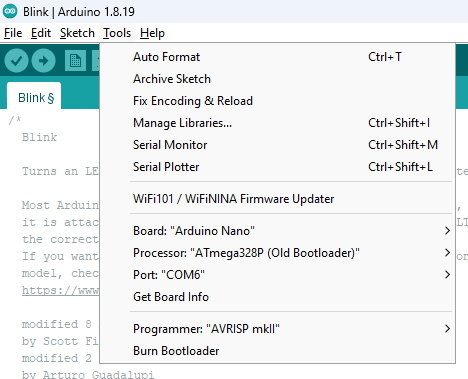
\includegraphics[width = 0.4\textwidth]{images/ArduinoReady.png}
    \cprotect\caption{A properly configured Arduino IDE. Note that the ``Port'' value will be different.}
\end{figure}

\newpage

\section{Background}

The goal of this lab is to get you acquainted with prototyping with Arduinos. First, you must understand the hardware you are working with. Next, you will learn how to write and upload software onto an Arduino. Finally, we will give a brief introduction into the Arduino programming language. At the end, you will be tasked with implementing some basic circuits involving LEDs, resistors, and pushbuttons.

\subsection{The Arduino Nano}

{\bf Figure 2} depicts the pinout diagram for the Arduino Nano. The pinout diagram summarizes the capabilities of the Arduino Nano and depicts the mapping between the physical pins on the microcontroller and the aliases given to the physical pins in software. For example, the digital pin ``D2'' is represented by the integer ``2'' in an Arduino program. \par

For this lab, we will be primarily focused on the digital pins, D0 - D19. The digital pins operate in a binary fashion; they send and receive signals as a logical HIGH or a logical LOW. Since the Arduino Nano operates on 5V logic, logical HIGH corresponds to 5V, while logical LOW corresponds to 0V. \par


\begin{figure}[ht]
    \centering
    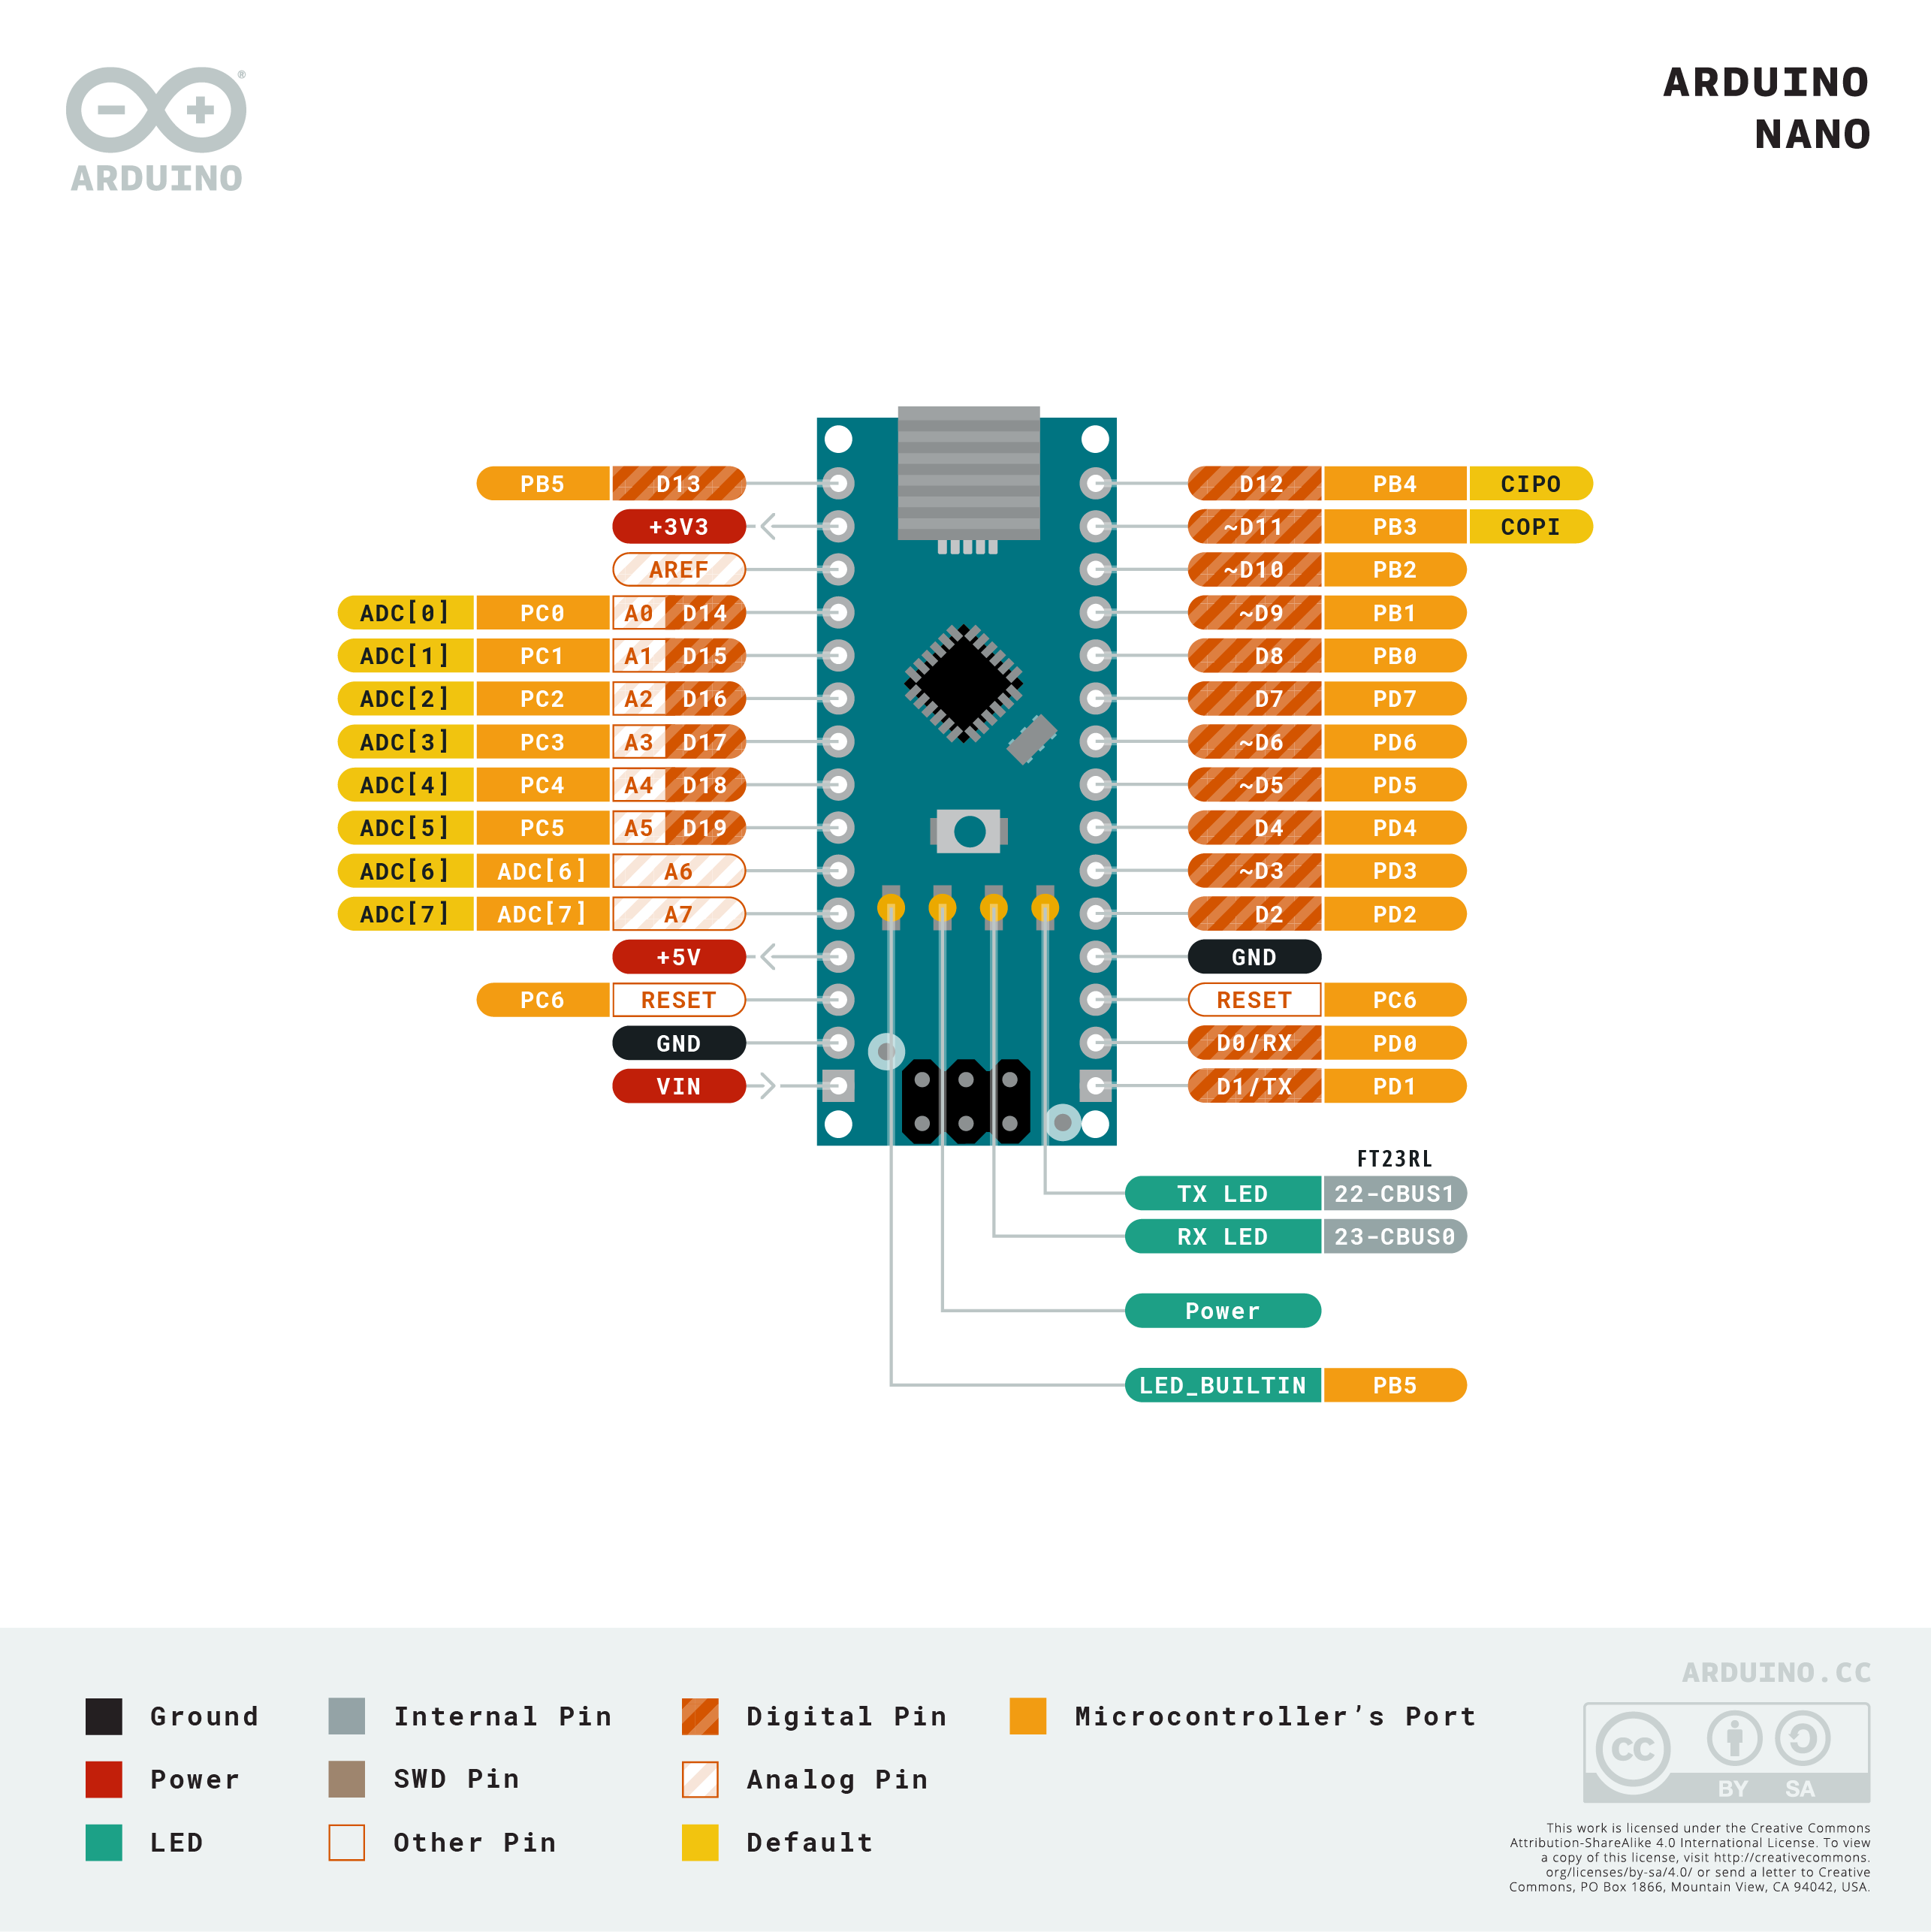
\includegraphics[width = 0.8\textwidth]{images/ArduinoNanoPinout.png}
    \cprotect\caption{Pinout for Arduino Nano. The ``Digital Pin'' numbers (D2, D3, etc...) 
    correspond to the numbers used in functions such as \verb|pinMode| and \verb|digitalWrite|.}
\end{figure}

\newpage

{\bf Figure 2} also depicts some pins that can't be interacted with via software, but are useful nonetheless. The +3V3 and +5V pins provide power, while the GND pins provide a ground reference. The VIN pin stands for ``Voltage In'', and it is used to supply 5V externally when you aren't providing the microcontroller power over USB. The ``Reset'' pins are used to restart the program on the Arduino Nano using an external signal. \par

The Arduino Nano also has some useful features besides its pins. The button in the middle of the Arduino Nano causes the program on the Arduino Nano to restart. The ``Power'' LED illuminates when the Arduino Nano is being powered by 5V. The LED labeled ``LED\_BUILTIN'' is an LED that can be controlled via software. You can address it using the \verb|LED_BUILTIN| macro in your program.

\subsection{Electrical Hardware}

The solderless breadboard shown in {\bf Figure 3} is your workspace when prototyping. The power rails labeled with ``+'' and ``-'' are connected horizontally and is ideal for distributing 5V and GND. The terminal strips in the middle of the solderless breadboard are connected vertically. The center divider separates the terminal strips on either side of breadboard from one another. \par

Jumper wires are useful for carrying electrical signals between different vertical terminal strips or between the power rails and the vertical terminal strips. Resistors are useful in conjunction with LEDs and pushbuttons. LEDs will burn themselves out if they are given too much current. The voltage drop across an LED is constant, so by increasing the resistance of the LED by using a resistor in series with an LED, the current drops. Resistors are also used with buttons to ensure the output of the button is never floating. See the appendix for more details.


\begin{figure}[ht]
    \centering
    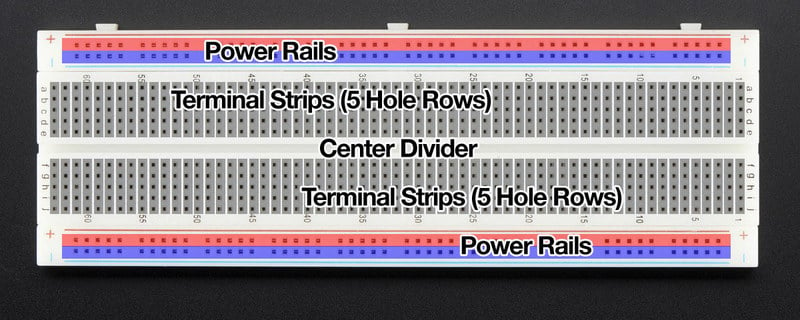
\includegraphics[width = 0.5\textwidth]{images/breadboard_diagram.jpg}
    \cprotect\caption{Anatomy of a solderless breadboard.}
\end{figure}

\begin{figure}[ht]
    \centering
    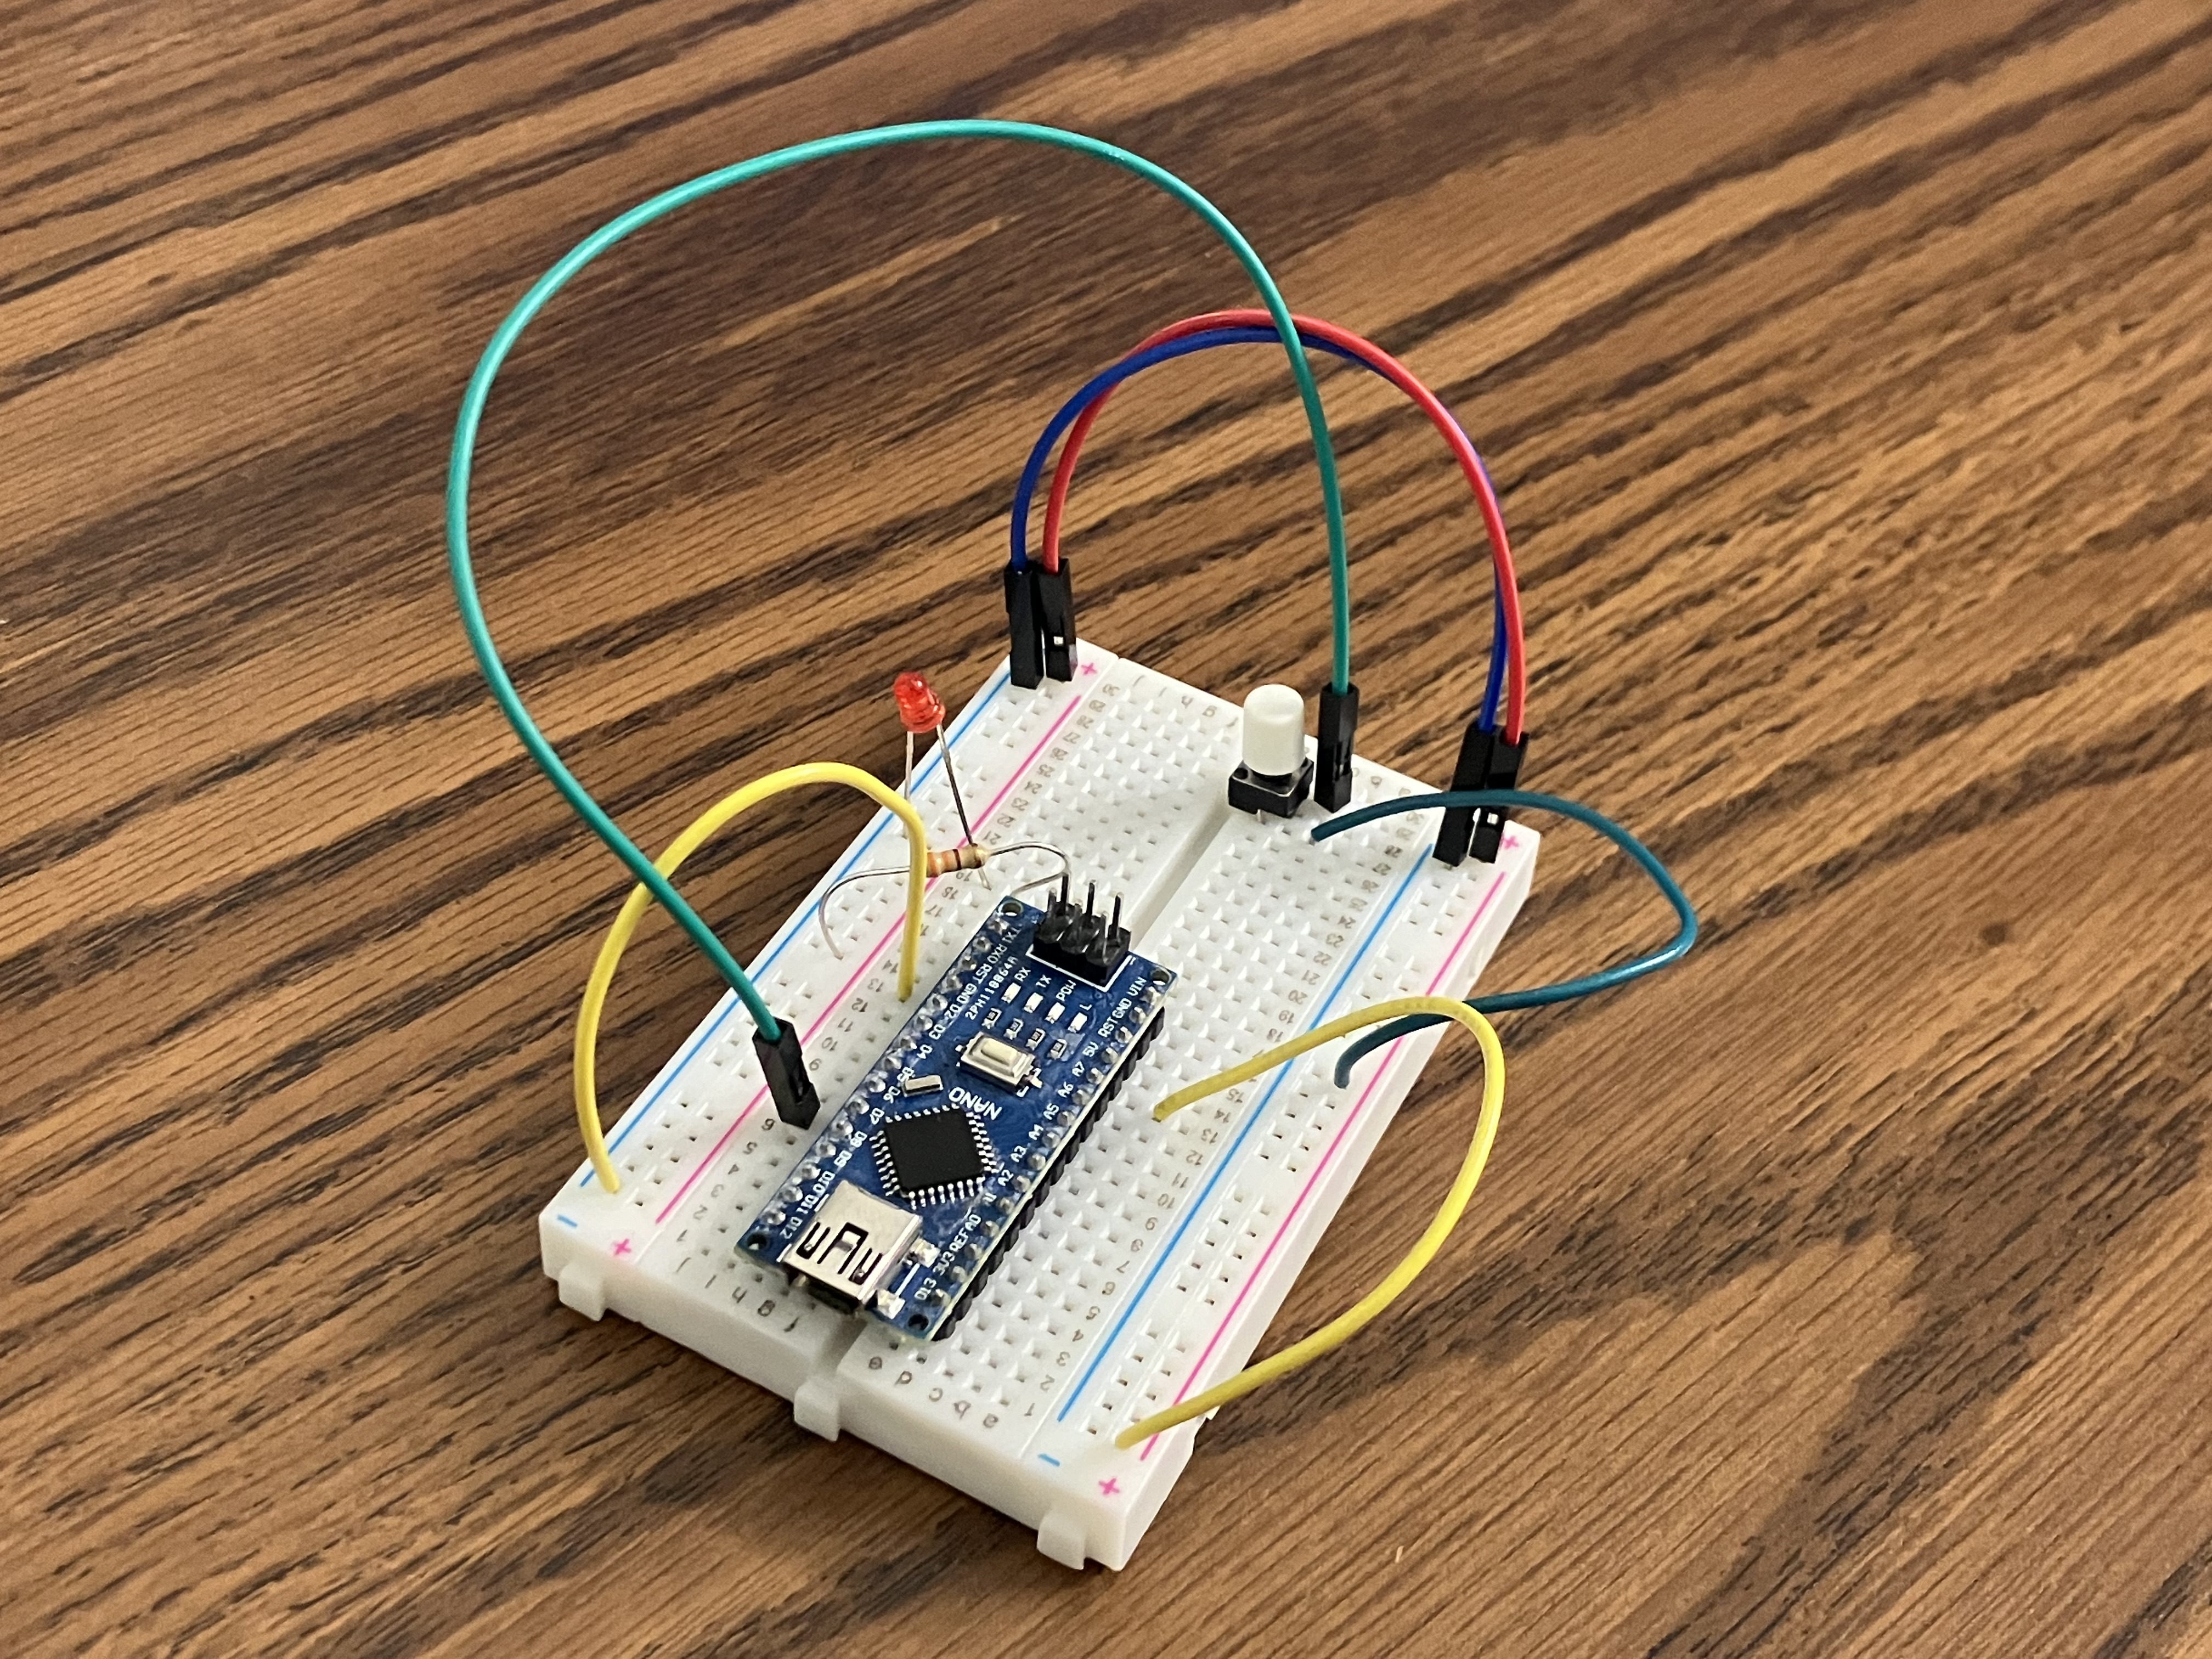
\includegraphics[width = 0.5\textwidth]{images/breadboard_example.jpg}
    \cprotect\caption{An example of how to lay out a circuit on a breadboard. The Arduino Nano straddles the center divider, providing power to the power rails. The resistor, LED, and button are laid out across different terminal strips and are connected using jumper wires.}
\end{figure}

\clearpage

\subsection{The Arduino IDE}

We will summarize a couple of important features for getting started with the Arduino IDE.

\subsubsection{Sketches and Examples}

User-created programs in the Arduino IDE are called sketches. The Arduino IDE also provides some built-in example sketches under File $>$ Examples. Some useful examples for this lab are ``Blink'' under ``Basics'' and ``Button'' under ``Digital''. You cannot modify examples, but you can use them as a starting points for your sketches.

\begin{figure}[ht]
    \centering
    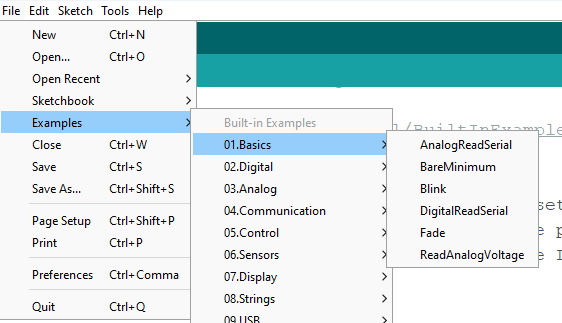
\includegraphics[width = 0.5\textwidth]{images/examples.png}
    \cprotect\caption{Accessing the Arduino IDE's built-in examples under File $>$ Examples.}
\end{figure}

\subsubsection{Verifying and Uploading Code}

Once you have written your Arduino program, you have to do two things before your code is running on the Arduino Nano.

\begin{itemize}
    \item {\bf Verify (checkmark button)}: This compiles your code into an executable format for the microcontroller. Compilation will fail if you have made a syntax error in your program. You do not need to be plugged into the microcontroller to Verify your program.
    \item {\bf Upload (arrow button)}: This uploads your code onto the microcontroller plugged into your computer. Uploading may fail if your settings in the ``Tools'' menu is incorrect; if you are having issues uploading to the microcontroller, go back to Section 1.2 and verify your settings are correct! The program will begin running immediately after it finishes uploading.
\end{itemize}

\begin{figure}[ht]
    \centering
    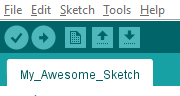
\includegraphics[width = 0.4\textwidth]{images/verifyupload.png}
    \cprotect\caption{The Verify (checkmark) and Upload (rightward-facing arrow) buttons in the Arduino IDE.}
\end{figure}

\clearpage

\subsubsection{The Arduino Programming Language}

The Arduino Programming language is similar to C++. Below, we have listed some useful functions for this lab:

\begin{itemize}
    \item \verb|setup()|: \verb|setup()| is called when the program starts. It will run once when you power on or reset the Arduino. \verb|setup()| is ideal for initializing variables and setting pin modes.
    \item \verb|loop()|: This function loops consecutively so the code you place here will constantly run. You can have other functions in your program but they will not run unless they are called in setup() or loop().
    \item \verb|pinMode(pin, mode)|: Configures \verb|pin| to behave as input or output.
    \begin{itemize}
        \item Example 1: \verb|pinMode(2, OUTPUT)| configures pin D2 on the Arduino Nano as an output.
        \item Example 2: \verb|pinMode(7, INPUT)| configures pin D7 on the Arduino Nano as an input.
        \item Example 3: \verb|pinMode(LED_BUILTIN, OUTPUT)| configures the built-in LED of the Arduino Nano as an output.
    \end{itemize}
    \item  \verb|digitalWrite(pin, value)|: Writes a HIGH or LOW value to a digital \verb|pin|.
    \begin{itemize}
        \item Example 1: \verb|digitalWrite(2, HIGH)| drives pin D2 to logical high (5V on Arduino Nano)
        \item Example 2: \verb|digitalWrite(2, LOW)| drives pin D2 to logical low (0V on Arduino Nano)
        \item Example 3: \verb|digitalWrite(2, 1)| drives pin D2 to logical high (5V on Arduino Nano)
    \end{itemize}
    \item \verb|digitalRead(pin)|: Reads a value (HIGH or LOW) from a digital \verb|pin|.
    \begin{itemize}
        \item Example 1: \verb|int buttonVal = digitalRead(7)| reads a digital value (\verb|HIGH=1| or \verb|LOW=0|) from pin D7 into the variable $\verb|buttonVal|$. 
    \end{itemize}
    \item \verb|delay(time)|: Pauses the program for a number of milliseconds.
    \begin{itemize}
        \item Example 1: \verb|delay(500)| pauses the program for 500 milliseconds.
    \end{itemize}
\end{itemize}

{\bf If you need information or examples on how the Arduino programming language works,}
\begin{itemize}
    \item Check out the \href{https://www.arduino.cc/reference/en/}{Arduino Language Reference}.
    \item Refer to the Arduino IDE's built-in Examples under File $>$ Examples. 
\end{itemize}

\clearpage

\section{Objective}

Here are some challenges for you to try out!

\subsection{Uploading Blink}

\begin{itemize}
    \item Open up the example Blink program under Files $>$ Examples $>$ Basics $>$ Blink.
    \item Verify and Upload the Blink program.
    \item The Arduino Nano's onboard LED should blink on and off.
\end{itemize}

\subsection{Blinking an External LED}
\begin{itemize}
    \item Create a sketch that will blink an LED on the breadboard.
    \begin{itemize}
        \item Refer to the Arduino Nano's pinout in section 2.1 to figure out which physical pins map to which numbers in software.
        \item You will need to use the \verb|pinMode|, \verb|digitalWrite|, and \verb|delay| functions. Refer to section 2.3.3 to learn how to use these functions.
    \end{itemize}
    \item You will need to put a resistor and LED in series, as shown in {\bf Figure 7}.
    \begin{itemize}
        \item LEDs have polarity; current will only flow from the anode (longer, positive leg) to the cathode (shorter, negative leg).
        \item Provide power through your software-controlled digital output pin on the Arduino Nano, and connect the LED's cathode (shorter, negative leg) to the Arduino Nano's GND. 
    \end{itemize}

    \begin{figure}[ht]
        \centering
        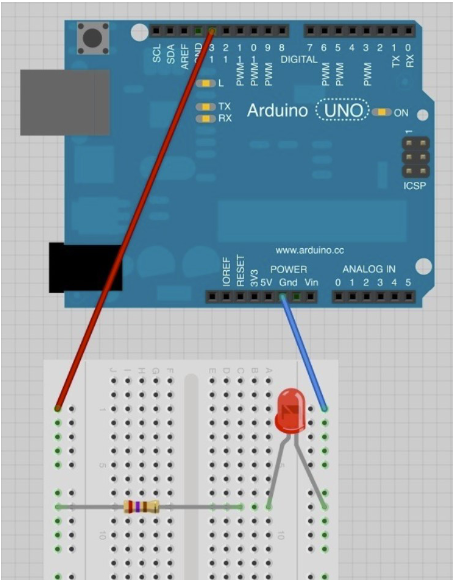
\includegraphics[width = 0.4\textwidth]{images/blinkLEDcircuit.png}
        \cprotect\caption{Example circuit diagram for blinking an external LED using an Arduino Uno. The resistor and LED are connected in series. Power is supplied through pin 13, and the LEDs cathode is connected to ground.}
    \end{figure}
    
\end{itemize}

\clearpage

\subsection{Blinking LEDs using a button}

\begin{itemize}
    \item Use the \verb|digitalRead| function to read the value of the button.
    \begin{itemize}
        \item To figure out how to wire up the button, refer to the Appendix.
    \end{itemize}
    \item Try controlling two different LEDs using two different digital output pins with the button. For instance, one LED could turn on while the other turns off when the button is pressed.
\end{itemize}

\subsection{Using button to adjust blink frequency (optional challenge)}

\begin{itemize}
    \item Use a button to control the rate at which an LED blinks.
    \item For instance, button unpressed = slow blink, button pressed = fast blink.
\end{itemize}

\subsection{Binary Counter (optional challenge)}

\begin{itemize}
    \item Create a binary counter using the button as input and the LEDs as output.
    \begin{itemize}
        \item A button press increments the count by 1
        \item Read up on \href{https://www.clivemaxfield.com/coolbeans/masking-and-the-c-c-bitwise-operators/}{Binary number and bit masking} to figure out how to translate a number into the LED output.
        \item Read the Appendix section about button debouncing
    \end{itemize}
\end{itemize}

\clearpage

\section{Appendix}

\subsection{Pull-up Resistors}

Pull-up resistors (and pull-down resistors) are used to ensure that a pin is not left floating when a connection is opened (by a button in this case). We connect the output side of the circuit to power through a resistor to accomplish this. Check out the circuit below. 

\begin{figure}[ht]
    \centering
    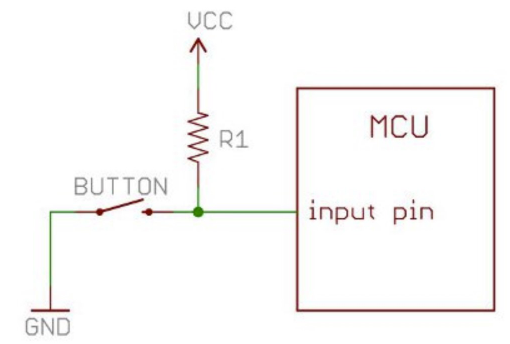
\includegraphics[width = 0.4\textwidth]{images/pullup.png}
    \cprotect\caption{Circuit diagram of pullup resistor in use with a button. When button is unpressed, resistor ``pulls up'' value of input pin. }
\end{figure}

Luckily, the Ardunio Nano has built-in pull-up resistors for all its digital pins, but we must activate them in firmware. To do this, we simply change the \verb|pinMode| of the pin. Instead of using \verb|pinMode(pin, INPUT)|, we use \verb|pinMode(pin, INPUT_PULLUP)|. You can read more \href{https://docs.arduino.cc/tutorials/generic/digital-input-pullup}{here}.

\subsection{Debouncing}

Due to mechanical/electrical issues, when a button is pressed it may be detected as many button presses.

\begin{figure}[ht]
    \centering
    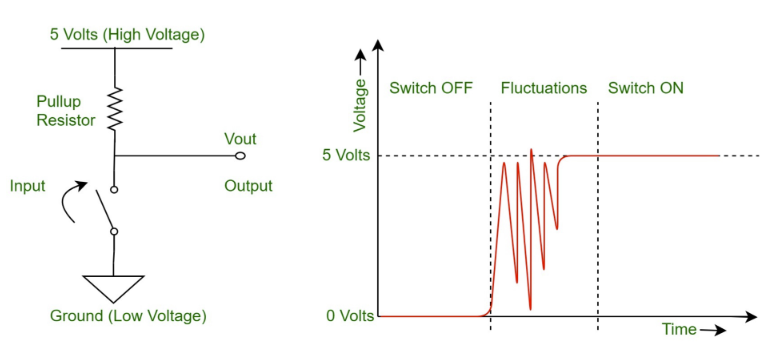
\includegraphics[width = 0.6\textwidth]{images/debouncing.png}
    \cprotect\caption{When switch is closed (left), voltage read by the microcontroller can fluctuate for a brief period before stabilizing (right). This can make a single button press look like several button presses.}
\end{figure}

These fluctuations might be detected by the MCU as many button presses, causing issues in firmware.
To counter this issue, there a few things we can do. For now, we can simply add a delay after we detect the change of state. However you decide to detect a button press to increment the binary counter, you can add a \verb|delay(50)| after so that the MCU doesn’t even look for another change of state until the delay is over. 50 ms is more than enough time to counter this issue.


\end{document}